\documentclass{article}
\usepackage{amsmath}
\usepackage{graphicx}
\bibliographystyle{IEEEtran}
\usepackage{caption}
\usepackage{subcaption}
\usepackage{geometry}
\usepackage[colorlinks=true]{hyperref}
\title{Author Response to Reviewers for the paper `Reducing object prior-bias in sparse projection tomographic reconstructions'}
\begin{document}
\maketitle

We thank all the reviewers for their detailed feedback on our work. Based on their comments, we have incorporated changes in our revised paper, and have discussed these in this document.


\section{Comments from AE}

\textcolor{blue}{\textit{While the reviewers have acknowledged improvements compared to the earlier manuscript, they have raised some important concerns about the manuscript in its current form. While addressing each of the reviewer specific comments, please pay specific attention to the following:}}

  \begin{itemize}
  \item \textcolor{blue}{\textit{Characterization of deep learning methods and its relation to the presented work}}

    We have now included a discussion of deep-learning methods in `Related Work', Section 2, of our paper, and have cited a few notable references pertaining to training neural networks to directly predict full-view sinogram and reconstruct the test object from its limited-view measurements.

    \item\textcolor{blue}{\textit{Presenting all relevant details so the work in the paper can be re-produced without ambiguity}}
      

      To ensure reproducibility, we had earlier shared the code files for 2D reconstructions. We have now added complete code 3D reconstructions as well in our github repository: \url{https://github.com/preetigopal/Weighted-Prior-Tomographic-Reconstruction.}

  \end{itemize}

  \section{Recommendation R1: AQ - Publish With Minor, Required Changes}

  \textbf{Comments:}The authors have significantly improved their paper when compared to the earlier rejected submission. The results are now much clearer. I have a few relatively minor comments below.\\

  \textcolor{blue}{\textbf{[R1-1,2; re-wording abstract]:}\textit{In the abstract, I feel you are underselling your contributions. You may want to add a line or two that quantifies the fidelity of your reconstructions for a given percentage of the total number of views (as required by Nyquist sampling). Your method is very relevant for scenarios such as Flash X-ray CT where we only are able to measure 5-20 views. Hence, some quantifying statement that appeals to the very few view CT community may be useful. In the abstract, the sentence "In this work, we mitigate this problem by first estimating the location of new regions and then imposing object-prior in only old regions which are similar to the prior." introduces terms such as "new regions" and "old regions" that don't carry any meaning. Please rewrite.}}\\

  \textbf{Response:} The reason we didn't specify quantitative results in the abstract is its dependency on various factors such as the number of views and structural complexity of the object data itself. We have however mentioned the importance of estimating a weights-map that shows the location and intensity of new regions. Meaning of the terms `old regions' and `new regions' have also been clarified in the new abstract.\\


  \textcolor{blue}{\textbf{[R1-3]:}\textit{In page 3 and lines 50-53 right column, you mention that your code will be released. However, I recommend including a link to github or other website with the code before publication.}}\\

  \textbf{Response:} Earlier, we had shared the complete code for 2D reconstruction. We have now added code for 3D reconstructions as well in the github repository: \url{https://github.com/preetigopal/Weighted-Prior-Tomographic-Reconstruction.}\\

  \textcolor{blue}{\textbf{[R1-4]:}\textit{In page 7 and lines 39-42 left column, what are the weights for? I don't see any equation where these can be substituted for quantifying results. Also, RMSE and SSIM have their own definitions.}}\\

  \textbf{Response:} Our earlier usage of the term `weights' with respect to SSIM might have been confusing since we also refer to `weights-map' throughout our paper. We have used the commonly used SSIM metric, for which, we have now provided reference to the original paper where the metric has been defined. SSIM comprises of three factors: Luminance, Contrast and Structure. These factors (called `coefficients' in our paper) for these three terms are adjustable to suit the application at hand. A description of computation of SSIM for a 2D image is given below. (The same formula can be extended to 3D.)

With $\mu_x$, $\mu_y$ and $\sigma_x^2$, $\sigma_y^2$ being the averages and variances of pixel values along dimensions $x$ and $y$ respectively, $\sigma_{xy}$ being the covariance along $x$ and $y$, $L$ being the dynamic range, $c_1$ and $c_2$, and $c_3$ being defined to be $(k_1L)^2$, $(K_2L)^2$ and $c_2/2$ repectively, with $k_1=0.01$ and $k_2=0.03$, the three components of SSIM metric: luminance $l$, contrast $c$ and structure $s$ are defined as: 

\begin{equation}
l(x,y) = \frac{2\mu_x\mu_y + c_1}{\mu_x^2 + \mu_y^2 + c_1}
\end{equation}

\begin{equation}
  c(x,y) = \frac{2\sigma_x\sigma_y + c_2}{\sigma_x^2 + \sigma_y^2 + c_2}
\end{equation}

\begin{equation}
  s(x,y) = \frac{\sigma_{xy} + c_3}{\sigma_x\sigma_y + c_3}
\end{equation}

Fianlly, SSIM is defined as

\begin{equation}
  SSIM = \frac{1}{n}\sum_x\sum_y [l(x,y)^\alpha. c(x,y)^\beta. s(x,y)^\gamma],
\end{equation}

where $n$ denotes the total number of pixels. The coefficients $\alpha$, $\beta$ and $\gamma$ are generally set to $1$ but are adjustable to suit the application goal.\\

\textcolor{blue}{\textbf{[R1-5, 6 (on Hyper-parameters)]:}\textit{In page 7 and lines 52-56 left column, I don't understand your tuning of $\lambda_1$. How is SSIM optimized when ground-truth is unknown for the test volume?
    It appears that the weight $\lambda_2$ must be chosen carefully and sufficiently high to ensure that we achieve the very fidelity reconstruction shown in Fig. 11 (h) with just 6 views. A lower incorrect choice for $\lambda_2$ will certainly bring back the artifacts. Even the parameter k probably plays an important role in achieving Fig. 11(h). Thus, your explanation for choosing $\lambda_2$ (in page 7 and lines 8-10 right column) and k (in page 7 and lines 23-27 right column) is inadequate. If you base your choice of $\lambda_2$ and k on "tolerance for noise" and/or "artifacts", how do you even quantify the relevant noise and artifacts? If $\lambda_2$ and k are chosen incorrectly, I am sure your method won't work. Hence, this detail needs to be discussed.}}\\

\textbf{Response:} Since the aim of our experiments is to demonstrate the benefit of using weighted prior reconstruction, we adjust these parameters by assuming the ground-truth to be known. However, we do not assume the Region Of Interest (RoI) of the test to be known.

We note that in practice, however, since ground-truth will never be
available, these parameters must be tuned using only the set of
templates available.  One of the templates can be assumed to be a
pseudo-test, and a grid search can be performed to get the best
possible hyperparameter values. These values can then be used for
reconstructing the `real' test volume.

As mentioned in Sec.6-B of the paper, $\lambda_1$ was tuned to maximize the SSIM of the complete reconstructed test volume using the TV-only regularizer. With the already chosen optimal $\lambda_1$, we apply our method for a range of $\lambda_2$ values and select the one that gives the best SSIM with reference to the ground truth.

As far as the stability of parameter $k$ is concerned, in Fig. 8 of our paper, we show how the quality of reconstructions vary for different values of $k$. We see that the reconstructions are similar for a significant range of $k$ values. (5-40) for Okra. For the purposes of demonstrating the benefit of our method, we choose $k$ omnisciently assuming known ground truth of test (and unknown RoI). In real-world, $k$ must also be tuned by using one of the templates as pseudo-test and performing a grid search to select the best value.\\


\section{Recommendation R2: RQ - Review Again After Major Changes}

\textbf{Comments:}The paper has greatly improved with the new focus! I would like to thank the authors for the extra work. I do have a few remaining comments:\\

\textcolor{blue}{\textbf{[R2-1]:}\textit{I highly suggest to use standard metrics for comparison, instead of the custom metrics currently used. For SSIM, reporting with the standard weightings is important (if the authors want, of course they can show both the standard weightings and the custom ones!). For RSME, I don't understand why the authors rescale images before computing the metric -- this can greatly alter the metrics, making them difficult to interpret and compare across papers. For the RMSE, it is best to not use any scaling at all (or, a fixed scaling for all reconstructions only based on the ground truth).
}}\\

\textbf{Response}:
Since SSIM inherently offers a flexibility to set coefficients based on what we want to evaluate, we believe that having a set of coefficients that focus on measuring structural preservation is better suited for our goal. However, in the paper, we have now included quantitative results with both custom (structure-focussed) SSIM and default SSIM. The benefit of the proposed method is seen with either setting of the metric.\\


\textcolor{blue}{\textbf{[R2-2]:}\textit{The computation comparison is not very convincing to me. In practice, given a certain number of projections, a user might want to compare possible reconstruction algorithms to decide what is the best one to use from a computation time / reconstruction quality tradeoff point of view. Therefore, it would be good to compare times between methods for the same number of projections (it is of course possible to show results for a few different cases, e.g. many views, moderate views, and few views). It is also useful to include more detailed information about the data size (detector size, reconstruction size, number of projections, etcetera). Furthermore, please show timing results for all steps of the algorithm, including the computation of the low quality reconstructions, pilot reconstructions, and building of eigenspaces.}}\\

\textbf{Response}: Earlier, we had indeed measured all computation times for exactly the same number of views. However, field-titles of Table-6 may not have been clear in this regard. Hence, we have edited the caption and Table-field titles of Table-6 (Page 10) to accurately describe details of measurement. Here, computation times of all methods and stages of reconstructions are measured for 30 views for  Liver slice of size $(512 \times 512)$.

Additionally, the TV reconstruction is our pilot reconstruction and hence their computation times are equal.

Having specified the exact compute times in our machine, we also note that the type of machine and the degree of parallelism available in the current times make these timing measurements, especially for iterative solutions, very subjective.
\\

\textcolor{blue}{\textbf{[R2-3]:}\textit{In several parts of the paper, the authors claim that existing object-prior based methods have problems, e.g.: "A common problem with these techniques is the strong influence of object-priors in the reconstruction of new regions in the test". At the moment, this hard claim is not supported in the paper by references or (even better) comparison results. It would be good to show, on one (or more) of the datasets used, that this is indeed the case, and that the proposed methods solves this problem.}}\\

\textbf{Response:}We have now included a reference (Pg.2, Line 3 under Sec.1-A) to a PhD thesis wherein the problem of object-priors biasing the reconstruction of new test regions is discussed in detail. 
A sample result (Fig.1-3 here) from the thesis is shown below. It illustrates how an unweighted application of prior can adversely affect the reconstruction of new regions in the test.\\

\begin{figure}[!h]
    \begin{subfigure}[b]{0.19\linewidth}
        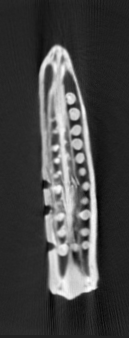
\includegraphics[width=\textwidth]{../images/thesis/okra/templateCropped_1.png}
\captionsetup{labelformat=empty}       
 \caption{}
    \end{subfigure}
    \begin{subfigure}[b]{0.19\linewidth}
        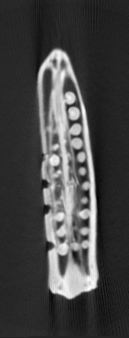
\includegraphics[width=\textwidth]{../images/thesis/okra/templateCropped_2.png}
\captionsetup{labelformat=empty}
        \caption{}
     \end{subfigure}
    \begin{subfigure}[b]{0.19\linewidth}
        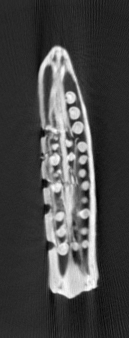
\includegraphics[width=\textwidth]{../images/thesis/okra/templateCropped_3.png}
\captionsetup{labelformat=empty}
        \caption{}
     \end{subfigure}
    \begin{subfigure}[b]{0.19\linewidth}
        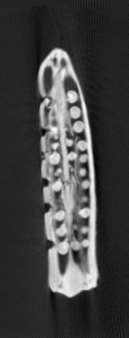
\includegraphics[width=\textwidth]{../images/thesis/okra/templateCropped_4.png}
\captionsetup{labelformat=empty}
        \caption{}
     \end{subfigure}
    \begin{subfigure}[b]{0.186\linewidth}
        \fcolorbox{yellow}{yellow}{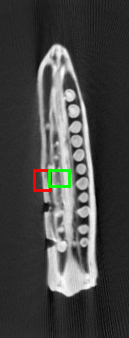
\includegraphics[width=\textwidth]{../images/thesis/okra/testCropped.png}}
\captionsetup{labelformat=empty}
        \caption{}
     \end{subfigure}
     \caption[Okra 3D dataset]{Okra 3D dataset: One slice each from the templates (the
       first four from the left), and one from the test volume
       (extreme right). In the regions marked in red and green, while
       all slices have deformities, the test
       has none.}
\label{fig:templates_test_okra}
\end{figure}
%----------------------------------------------------

\begin{figure}[!h]
\centering
\subcaptionbox{Test}{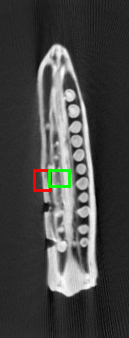
\includegraphics[width=0.19\columnwidth]{../images/thesis/okra/testCropped.png}}\hfill
\subcaptionbox{FDK}{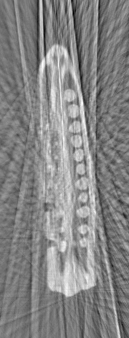
\includegraphics[width=0.19\columnwidth]{../images/thesis/okra/fdk_cropped.png}}\hfill
\subcaptionbox{Sparsity prior}{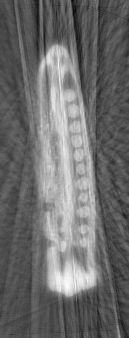
\includegraphics[width=0.19\columnwidth]{../images/thesis/okra/cs_cropped.png}}\hfill
\subcaptionbox{Sparsity and \\unweighted \\template priors}{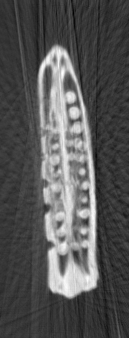
\includegraphics[width=0.19\columnwidth]{../images/thesis/okra/pca_cropped.png}}\hfill
\subcaptionbox{Sparsity and \\weighted template\\ priors}{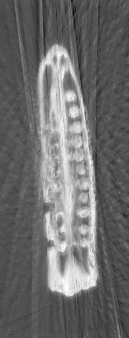
\includegraphics[width=0.19\columnwidth]{../images/thesis/okra/prior_weighted_cropped.png}}
\caption[3D reconstruction of okra dataset]{3D reconstruction of the okra from $10\%$ projection
  views (b) has strong streak artefacts, (c) blurred, (d) no new
  information detected (prior dominates -- the deformity from the prior
  shows up as a false positive) and (e) new information detected (no deformities
  corresponding to red and green regions) while simultaneously
  reducing streak artefacts.}
\label{fig:okra_3D_results}
\end{figure}

%--------------------------------------zoomed okra

\begin{figure}[!h]
\centering
\subcaptionbox{Test}{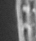
\includegraphics[width=0.19\columnwidth]{../images/thesis/okra/zoomed/input_cropped.png}}\hfill
\subcaptionbox{FDK}{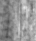
\includegraphics[width=0.19\columnwidth]{../images/thesis/okra/zoomed/FDK_cropped.png}}\hfill
\subcaptionbox{Sparsity prior}{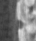
\includegraphics[width=0.19\columnwidth]{../images/thesis/okra/zoomed/pca_cropped.png}}\hfill
\subcaptionbox{Sparsity and \\unweighted \\template priors}{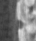
\includegraphics[width=0.19\columnwidth]{../images/thesis/okra/zoomed/pca_cropped.png}}\hfill
\subcaptionbox{Sparsity and \\weighted template\\ priors}{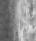
\includegraphics[width=0.19\columnwidth]{../images/thesis/okra/zoomed/weighted_prior_cropped.png}}
\caption[Zoomed results of Okra dataset]{Zoomed in portion corresponding to the red RoI of Fig.~\ref{fig:okra_3D_results} for various methods (b) has strong streak artefacts, (c) blurred, (d) no new  information detected (prior dominates -- the deformity from the prior
  shows up as a false positive) and (e) new information detected (no deformities
 ).}
\label{fig:okra_zoomed_3D_results}
\end{figure}

\textcolor{blue}{\textbf{[R2-4]:}\textit{The discussion of deep learning methods in Section 7B is not very strong in my opinion. There are many existing techniques that have shown quite convincing results for reconstructing CT images with a low number of projections, even without taking into account any static parts across time. These methods rely on learning image-based correlations instead of the "given intensities of a voxel at various time instants in a longitudinal setting and partial measurements of the voxel at the current time, what will be the intensity of the same voxel at the current time instant?" given by the authors. These image-based methods often don't need 'hundreds of labeled data', sometimes being able to accurately learn from just one time step. In the paper, these methods should be discussed, and proper references should be included.}}\\

\textbf{Response}: We acknowledge that there has been significant work pertaining to training neural networks to directly predict full-view sinogram and reconstruction of the test object from its limited-view measurements. We have now included a discussion of deep-learning methods in `Related Work', Section 2, of our paper, and have now cited a few notable references.

We also believe that information from longitudinal data, if available, is helpful and must be used to better inform reconstruction of the test. This is especially the case in applications where longitudinal data is naturally available as part of the process as in radio frequency ablations. It is in this context that our paper presents an analytical method to fuse the existing prior data with test measurements in order to construct a `weights map'. This map gives clear insights about regions of change within the object over time.\\



\textcolor{blue}{\textbf{[R2-5]:}\textit{What algorithm is used to minimize Eq 3? How many iterations were used for this minimization? How was convergence ensured?}}\\

\textbf{Response}: Eq. 3 consists of alternately solving for Eq.4 and Eq.5. While Eq.5 has a closed form solution, Eq.4 was solved using the solver mentioned in Reference [18]. (as mentioned in page 6, just above Eq.4). 
For solving Eq.4, maximum number of iterations was set to 200 and tolerance was set to 1e-4.

The number of alternate minimization cycles (between Eq.4 and~5) was set to 3. We observed that further cycles did not improve reconstruction significantly for the extra time consumed.
\\

\textcolor{blue}{\textbf{[R2-6]:}\textit{What were the various parameters of the reconstructions show in Fig 11? How were they chosen?
}}\\

\textbf{Response}: For 2D reconstructions using ART, SIRT and SART, we set the maximum iterations to 50 and observed that further iterations did not improve the quality of reconstructions.\\

\textcolor{blue}{\textbf{[R2-7]:}\textit{How was the $\lambda_2$ parameter empirically chosen?
}}\\

\textbf{Response}: Please refer to our response to a similar query in \textcolor{blue}{\textbf{[R1-5,6]}}.\\

\textcolor{blue}{\textbf{[R2-8]:}\textit{In some parts of the paper, the use of language could be improved. Also, I think it is better to not use words like `paltry'.}}\\

\textbf{Response}: Although we had meant to use `paltry' in a neutral way to only suggest the use of very few measuremetns, we  have noted this and made the change.\\

\section{Recommendation R3: RQ - Review Again After Major Changes}

\textbf{Comments:} The paper presents an image reconstruction method for recovering samples from limited projections provided that the high-quality CT-scans of the same sample exist. This approach could be useful to longitudinal studies in which the patient's previous CT scans are available and the purpose is to reduce the dose. So this is good!\\

The structure of the paper is good and the authors did a good job in presenting both the theory and the validation with experimental data, demonstrating the potential. of the nice things about the paper is that they use PCA to get the orthonormal basis to represent the image and this both serves as a regularizer as well as a nice way to quantify new features in data.
\\

\textcolor{blue}{\textbf{[R3-1]:}\textit{One challenge of the method that I can see is that these datasets needs to be aligned but there is not much discussion on this procedure or how this can be performed in a realistic setting. Are the variation from a past to present scans looking similar? In addition to the variations in scans taken at different times, in the low-quality scan, the features are less pronounced so the registration might pose a challenge even if the sample looks similar. So, it would be good to see the artifacts due to an intentionally less-aligned images and a discussion about the limitations would be nice.
}}\\

\textbf{Response}:Yes, registration between the unknown test and templates is important for our method. Registration is also a common problem in many other fields such as MRI/CT/PET data.  There is a lot of research on linear and non-linear methods to optimise this. The focus in our paper is not on registration but on building accurate maps that delineate regions of structural changes in already pre-registered data (registered using state-of-the-art methods).  Hence, in this work, we do not intend to predict what difficulties registration might present but rather that show that it is possible to blend prior and new views.\\

We note that in practice, a pilot reconstruction of the test must be registered with similarly imaged, pilot reconstructed templates. This registration is challenging due to the presence of sub-sampling artefacts. We consider the problem of registration as a separate one and intend the practitioners to use any state-of-the-art registration algorithm before applying the proposed method in our paper. 
\\

\textcolor{blue}{\textbf{[R3-2]:}\textit{Another challenge, as the authors acknowledge, is the high number of hyper-parameters. I believe the paper can benefit a lot from an in depth analysis to get some insights about how this parameters should be chosen. Because otherwise the applicability of the method is limited given the amount of time required to solve the reconstruction problem.
}}\\

\textbf{Response}: Please refer to our response to a similar query in \textcolor{blue}{\textbf{[R1-5,6]}}.\\


\textcolor{blue}{\textbf{[R3-3]:}\textit{The title says ``eliminating object prior-bias'', but I think this is not accurate, because you give a weight to those priors, but not fully eliminate them. A more appropriate wording might be ``Prior-informed sparse-projection...'' or ``Weighted object-priors from past CT-scans for ...'' or something like this.}}\\

\textbf{Response}: Thank you for suggesting other possible titles. We have changed it to ``Reducing object prior-bias from sparse-projection tomographic reconstructions''\\


\textcolor{blue}{\textbf{[R3-4]:}\textit{As a final remark, the authors can also use this technique for imaging dynamical samples. A discussion would be nice.}}\\

\textbf{Response}: Based on our understanding, dynamic imaging is a technique for acquiring only those measurements that have high entropy. This involves computing the next the measurement location based on the past measurements acquired for the \textit{same} object volume. This is different from our scenario in which we consider measurements from \textit{multiple volumes} of an object, each taken at a different time. The measurement-locations of the test are also not pre-computed while imaging, in our case. 

Hence, our method may not be directly applicable for reconstruction from dynamic imaging wherein the acquired measurements of a single object are already non-redundant by design. However, a suitable dynamic imaging reconstruction algorithm (like the Compressed Sensing)  can definitely be used as a pilot reconstruction method within our framework. 



    
  \end{document}


\bibliography{tci_ref}
\end{document}
\begin{table}[!h]
  \centering
\caption{Standard-SSIM (`SSIM-1'), structure-focussed SSIM (`SSIM-2') and RMSE of the reconstructions shown in Fig.11:(a)-(h) of the paper. %The SSIM of
                                %ideal reconstruction is 1. The ideal
                                %RMSE is 0, and the worst RMSE
                                %possible is 1 here.
}
\begin{tabular}{|l|c|c|c|c|c|c|c|c|c|}
\hline
& \textbf{(a)} & \textbf{(b)} & \textbf{(c)} & \textbf{(d)} & \textbf{(e)} & \textbf{(f)} &  \textbf{(g)} &  \textbf{(h)} \\\hline
SSIM-1 & 0.31 & 0.48  & 0.39  & 0.51 & 0.55  & 0.42 & 0.68 &\textcolor{red}{0.78} \\ \hline
SSIM-2 & 0.64 & 0.72  & 0.68 & 0.83 & 0.81 & 0.69 & 0.83 &\textcolor{red}{0.88} \\ \hline
RMSE & 0.38 & 0.18 & 0.25 & 0.43 & 0.33 & 0.21 & 0.11 & \textcolor{red}{0.04}\\ \hline
\end{tabular}
\label{table:potato_2D_ssim}
\end{table}
